\section{Theorie}
\label{sec:Theorie}
Dieser Versuch behandelt die Ablenkung von Elektronenstrahlen im B-Feld und
im E-Feld.
\subsection{Kathodenstrahlröhre}
Zur Untersuchung im elektrischen Feld wird eine Kathodenstrahlröhre genutzt,
dargestellt in Abbildung \ref{fig:krs}.
\begin{figure}
 \centering
 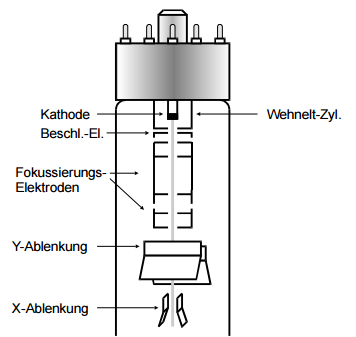
\includegraphics[width=0.5\textwidth]{krs.pdf}
 \caption{Queerschnitt einer Kathodenstrahlröhre.}
 \label{fig:krs}
\end{figure}
Die Röhre besteht im wesentlichen aus drei Komponenten, der "Elektronenkanone",
diese erzeugt, und beschleunigt freie Elektronen und
fokussiert den entstehenden Elektronenstrahl und einem
Ablenk- bzw. Nachweissystem.
Mittels Glühemission werden die freien Elektronen von einer Kathode, aus
einem Material mit kleiner Austrittsarbeit, erzeugt.
Die Kathode ist von einem sogenannten Wehnelt-Zylinder ummantelt, dieser enthält
eine Bohrung und weist ein negatives Potential auf, damit lässt sich die
Intensität des Elektronenstrahls steuern.
Eine Elektrode, mit hohem positivem Potential, befindet sich
vor dem Wehnelt-Zylinder. Die Elektrode beschleunigt diejenigen Elektronen,
welche den Wehnelt-Zylinder überwinden können.
Das Strahlenbündel wird mit einer elektronischen Linse, mittels
inhomogener elekrischer Felder, auf den einen Leuchtschirm fokussieren.
Die Brechkraft der Linse ist von  der Spannung $U_\mathrm{c}$ abhängig.
Zwei Plattenpaare, deren Normalen senkrecht aufeinander stehen, bilden
das Ablenksystem. Beim Anlegen einer Spannung wirkt wegen des E-Feldes
eine Kraft auf den Elektronenstrahl und es kommt zur Ablenkung.
Diese
